\documentclass[a4paper]{article}
\usepackage[french]{babel}
\usepackage{graphicx}
\title{ Tuned mass damper}
\author{FRAMBOURT Mateïs et BOCQUILLON Noé}

\begin{document}
	\maketitle
\paragraph{\underline{Titre provisoire:}} Modélisation et simulation d'un immeuble à amortisseur harmonique.
	
\paragraph{\underline{Objectif du TIPE:}}
  Mesurer et évaluer l'efficacité d'un amortisseur harmonique (Tuned mass Damper).
  
  \paragraph{\underline{Manipulations:}}
  Le but est dans un premier temps de modéliser par une maquette très simple un immeuble et de le faire entrer en vibration à l'aide d'un axe linéaire.
  Nous allons d'abord construire une maquette rigide afin de montrer que celle-ci vibrera à la même fréquence et amplitude que l'entrée et donc ne sera pas adapté à ce que l'on veut observer.De plus, cette première expérience sera l'occasion de vérifier que nos projets de modélisation de maquette sont réalisables ainsi que le bon fonctionnement de l'acquisition de données (L'acquisition sera décrite de manière plus précise plus bas)
 
\subparagraph{Description de la maquette:}Sur une base en bois, on fixe 4 tiges de bois rigides et épaisses dont le haut est relié par une plaque en bois %\input{./photo} 
\begin{figure}[h]
 \center{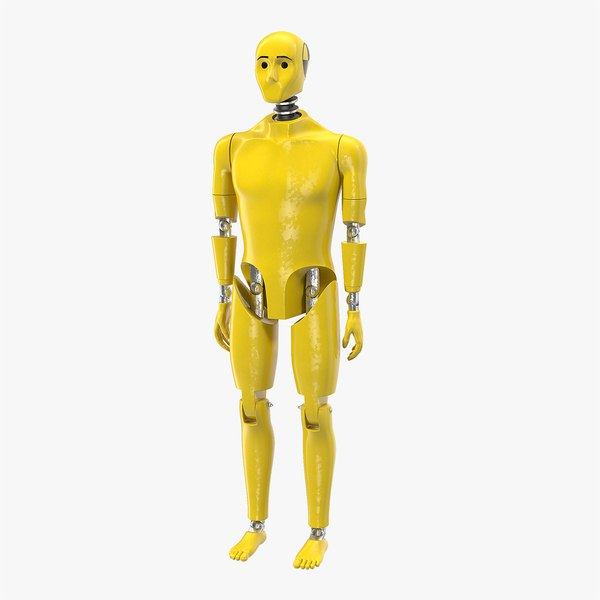
\includegraphics[scale=0.1]{dummy.jpg}}
 \caption {maquette de l'immeuble rigide}
\end{figure}

 
 
 
 
 
 \subparagraph{}Nous allons ensuite construire un modèle un peu plus représentatif des interactions réelles. Pour cela, nous visseront des demi-balles rebondissante à chaque liaison pour simuler une déformation avec une force de rappel. Cette modélisation permettra de (
\begin{figure}[h]
 \center{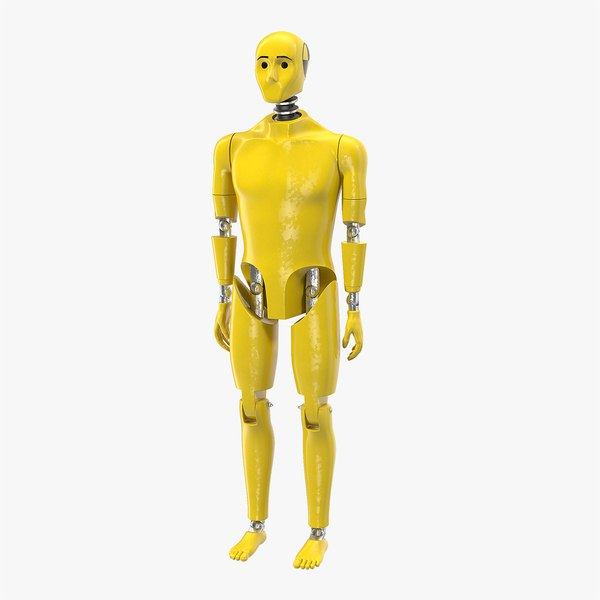
\includegraphics[scale=0.1]{dummy.jpg}}
 \caption {maquette de l'immeuble semi flexible}
\end{figure}
La maquette sera fixée sur un axe linéaire qui permet la mise en vibration. 
L'acquisition de l'accélération en fonction du temps sera effectuée dans un premier temps, de manière simple et intuitive , à l'aide de nos deux téléphones et de l'application \textit{Physics Tool Box} qui contient un accéléromètre. L'utilisation de nos deux téléphones (un fixé en haut et l'autre en bas)permettra de comparer la différence d'amplitude entre le haut et le bas de la maquette et une éventuelle résonance. Mais la masse de nos deux téléphone étant non négligeable, il sera envisagé de remplacer les téléphones par des modules accéléromètre et un microcontrolleur.
L'ajout d'en pendule simple fixé sur le haut de la structure devrait nous permettre d'observer une éventuelle réduction des oscillations en sa présence. 
 

\end{document}